% CAP description for Tree
A Tree is a component with linked
elements (nodes) and a hierarchical structure. One common example is
the display of directory structures used in most file managers
(e.g. \bxname{Windows Explorer}).

\begin{figure}
\begin{center}
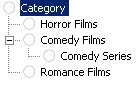
\includegraphics{PS/Tree}
\caption{Tree}
\label{tree}
\end{center}
\end{figure}


Because the forward slash (/) is a special symbol for trees, if you want to use a slash as part of your parameter value, you have to mask it. See the section later in this document \bxpref{specialchar} for more details. 

\textbf{Mapping trees}

In the \gdomm{}, a tree to be mapped looks like this:

\begin{figure}
\begin{center}
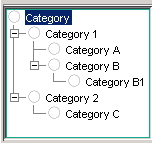
\includegraphics{PS/Maptree}
\caption{Tree}
\label{maptree}
\end{center}
\end{figure}

\bxtipp{Actions on trees (as a hierarchical component) are not supported in the HTML toolkit. Individual nodes must be addressed as single links.}
